\begin{name}
	{ÔN TẬP KIỂM TRA CUỐI HỌC KÌ 1}
	{TOÁN 10}
	{LỚP TOÁN THẦY PHÁT}
	{\thoigian}
\end{name}
%================================PHẦN I
\caulc
\Opensolutionfile{ans}[ans/0-HK1-CD-6-NgocTao-HaNoi-Phan-I]

% Phần I.Câu 1
\begin{ex}%[0-HK1-CD-6-NgocTao-HaNoi-2324]%[VN-MT-6, Bùi Lương Phúc]%[[0D1N1-5]]%[0D1N1-3]
Phát biểu mệnh đề phủ định của mệnh đề \lq\lq $\forall n\in \mathbb{N} \colon n^2-4n+7\ne 0$\rq\rq \ là
\choice
{\lq\lq $\exists n\in \mathbb{N} \colon n^2-4n+7\le 0$\rq\rq}
{\True \lq\lq $\exists n\in \mathbb{N} \colon n^2-4n+7=0$\rq\rq}
{\lq\lq $\forall n\in \mathbb{N} \colon n^2-4n+7=0$\rq\rq}
{\lq\lq $\exists n\in \mathbb{N} \colon n^2-4n+7\ne 0$\rq\rq}
\loigiai
{Mệnh đề phủ định của mệnh đề \lq\lq $\forall n\in \mathbb{N} \colon n^2-4n+7\ne 0$ \rq\rq \ là
\lq\lq $\exists n\in \mathbb{N} \colon n^2-4n+7=0$\rq\rq.}
\end{ex}

% Phần I.Câu 2
\begin{ex}%[0-HK1-CD-6-NgocTao-HaNoi-2324]%[VN-MT-6, Bùi Lương Phúc]%[0D1N1-1]
Trong các câu sau đây, câu nào là mệnh đề chứa biến?
\choice
{\lq\lq $\sqrt{3}$ là số vô tỉ\rq\rq}
{\lq\lq $2$ là số chẵn duy nhất\rq\rq}
{\True \lq\lq $x\in \mathbb{R}$, $x^2-1+x>0$\rq\rq}
{\lq\lq Hình thoi có hai đường chéo vuông góc với nhau\rq\rq}
\loigiai
{Mệnh đề chứa biến (biến $x$) là \lq\lq $x\in \mathbb{R}$, $x^2-1+x>0$\rq\rq. \\
Các câu còn lại là những mệnh đề.}
\end{ex}

% Phần I.Câu 3
\begin{ex}%[0-HK1-CD-6-NgocTao-HaNoi-2324]%[VN-MT-6, Bùi Lương Phúc]%[0D1N2-3]
Hình vẽ nào sau đây (phần không bị gạch) minh họa cho tập hợp $E=[-3;12)$?
\choice
{\begin{tikzpicture} [scale=0.2, font=\footnotesize, line cap = round, line join = roud, >=stealth]
\draw[->] (-8,-2)--(18,-2);
\fill[pattern=north east lines, opacity=0.7] (-8,-70pt) rectangle (-3,-40pt);
\fill[pattern=north east lines, opacity=0.7] (12,-70pt) rectangle (18,-40pt);
\path (-3,-2) node {$\big($} node[below = 6pt]{$-3$};
\path (12,-2) node {$\big)$} node[below = 6pt]{$12$};
\end{tikzpicture}}
{\True \begin{tikzpicture} [scale=0.2, font=\footnotesize, line cap = round, line join = roud, >=stealth]
\draw[->] (-8,-2)--(18,-2);
\fill[pattern=north east lines, opacity=0.7] (-8,-70pt) rectangle (-3,-40pt);
\fill[pattern=north east lines, opacity=0.7] (12,-70pt) rectangle (18,-40pt);
\path (-3,-2) node {$\big[$} node[below = 6pt]{$-3$};
\path (12,-2) node {$\big)$} node[below = 6pt]{$12$};
\end{tikzpicture}}
{\begin{tikzpicture} [scale=0.2, font=\footnotesize, line cap = round, line join = roud, >=stealth]
\draw[->] (-8,-2)--(18,-2);
\fill[pattern=north east lines, opacity=0.7] (-8,-70pt) rectangle (-3,-40pt);
\fill[pattern=north east lines, opacity=0.7] (12,-70pt) rectangle (18,-40pt);
\path (-3,-2) node {$\big[$} node[below = 6pt]{$-3$};
\path (12,-2) node {$\big]$} node[below = 6pt]{$12$};
\end{tikzpicture}}
{\begin{tikzpicture} [scale=0.2, font=\footnotesize, line cap = round, line join = roud, >=stealth]
\draw[->] (-8,-2)--(18,-2);
\fill[pattern=north east lines, opacity=0.7] (-8,-70pt) rectangle (-3,-40pt);
\fill[pattern=north east lines, opacity=0.7] (12,-70pt) rectangle (18,-40pt);
\path (-3,-2) node {$\big($} node[below = 6pt]{$-3$};
\path (12,-2) node {$\big]$} node[below = 6pt]{$12$};
\end{tikzpicture}}
\loigiai{
Tập hợp $E=[-3;12)$ có hình minh họa là
\begin{center}
\begin{tikzpicture} [scale=0.4, font=\footnotesize, line cap = round, line join = roud, >=stealth]
\draw[->] (-8,-2)--(18,-2);
\fill[pattern=north east lines, opacity=0.5] (-8,-70pt) rectangle (-3,-45pt);
\fill[pattern=north east lines, opacity=0.7] (12,-70pt) rectangle (18,-45pt);
\path (-3,-2) node {$\big[$} node[below = 6pt]{$-3$};
\path (12,-2) node {$\big)$} node[below = 6pt]{$12$};
\end{tikzpicture}
\end{center}
}
\end{ex}

% Phần I.Câu 4
\begin{ex}%[0-HK1-CD-6-NgocTao-HaNoi-2324]%[VN-MT-6, Bùi Lương Phúc]%[0D2N2-1]
Trong các hệ sau, hệ nào \textbf{không} phải là hệ bất phương trình bậc nhất hai ẩn?
\choice
{$\heva{&5x-4y\ge -1 \\&4x+5y\le 10}$}
{$\heva{&2x-y\ge -3 \\&x+3y\le 1}$}
{$\heva{&2x-y>-1 \\&-x+3y\le 5}$}
{\True $\heva{&x+y^2\le 1 \\&4x+5y>10}$}
\loigiai
{Hệ $\heva{&x+y^2\le 1 \\&4x+5y>10}$ không phải là hệ bất phương trình bậc nhất hai ẩn.}
\end{ex}

% Phần I.Câu 5
\begin{ex}%[0-HK1-CD-6-NgocTao-HaNoi-2324]%[VN-MT-6, Bùi Lương Phúc]%[0H4N1-3]
Cho $0^\circ <\alpha<180^\circ$. Trong các khẳng định sau, khẳng định nào đúng?
\choice
{$\cos (180^\circ -\alpha)=\cos \alpha$}
{\True $\sin (180^\circ -\alpha)=\sin \alpha$}
{$\cot (180^\circ -\alpha)=\cot \alpha$}
{$\tan (180^\circ -\alpha)=\cot \alpha$}
\loigiai
{Ta có
\begin{itemize}
\item $\cos (180^\circ -\alpha)=-\cos \alpha$;
\item $\sin (180^\circ -\alpha)=\sin \alpha$;
\item $\cot (180^\circ -\alpha)=-\cot \alpha$;
\item $\tan (180^\circ -\alpha)=-\tan \alpha$.
\end{itemize}
}
\end{ex}
% Phần I.Câu 6
\begin{ex}%[0-HK1-CD-6-NgocTao-HaNoi-2324]%[VN-MT-6, Bùi Lương Phúc]%[0H4H2-1]
Cho tam giác $ABC$ có $BC^2 + CA^2 - AB^2 < 0$. Khẳng định nào sau đây đúng?
\choice
{\True $\widehat{C}>90^\circ$}
{$\widehat{A}>90^\circ$}
{$\widehat{B}>90^\circ$}
{$\widehat{A}=90^\circ$}
\loigiai{
Theo định lý cosin, ta có
\begin{eqnarray*}
BC^2+CA^2-AB^2
&=& BC^2+CA^2-\left(BC^2+CA^2-2\cdot BC\cdot CA\cdot \cos C\right)\\
&=& 2\cdot BC\cdot CA\cdot \cos C.
\end{eqnarray*}
Vì $BC^2+CA^2-AB^2<0$ nên $\cos C<0$ hay $\widehat{C}>90^\circ$.
}
\end{ex}

% Phần I.Câu 7
\begin{ex}%[0-HK1-CD-6-NgocTao-HaNoi-2324]%[VN-MT-6, Bùi Lương Phúc]%[0H4N2-1]
Cho tam giác $ABC$ biết $BC = 6$, $\widehat{A}=120^\circ$. Tính bán kính $R$ của đường tròn ngoại tiếp tam giác $ABC$.
\choice
{$R=12$}
{$R=6$}
{\True $R=2\sqrt{3}$}
{$R=4\sqrt{3}$}
\loigiai{
Bán kính của đường tròn ngoại tiếp tam giác $ABC$ là $R= \dfrac {BC}{2 \sin A}=\dfrac {6}{\sqrt {3}}=2\sqrt{3}$.}
\end{ex}

% Phần I.Câu 8
\begin{ex}%[0-HK1-CD-6-NgocTao-HaNoi-2324]%[VN-MT-6, Bùi Lương Phúc]%[0H5H4-1]
Cho tam giác $ABC$ đều. Góc giữa hai vectơ $\overrightarrow{AB}$ và $\overrightarrow{BC}$ là
\choice
{\True $120^\circ$}
{$60^\circ$}
{$30^\circ$}
{$150^\circ$}
\loigiai
{\begin{center}
\begin{tikzpicture}[scale=1, font=\footnotesize, line join=round, line cap=round, >=stealth]
\coordinate (A) at (0,0);
\coordinate (B) at (4,0);
\coordinate (C) at (2,{2*sqrt(3)});
\coordinate (D) at (8,0);
\draw (A) -- (B) -- (C) -- cycle;
\draw[->] (B) -- (D);
\foreach \x/\y in {A/0,B/0,C/100,D/0} \fill(\x) circle (1pt) ($(\x)+(\y:3mm)$) node[below left]{$\x$};
\end{tikzpicture}
\end{center}
Vẽ vectơ $\overrightarrow{BD}=\overrightarrow{AB}$.\\
Khi đó, góc giữa hai vectơ $\overrightarrow{AB}$ và $\overrightarrow{BC}$ bằng góc giữa hai vectơ $\overrightarrow{BD}$ và $\overrightarrow{BC}$ và bằng $120^\circ$.}
\end{ex}

% Phần I.Câu 9
\begin{ex}%[0-HK1-CD-6-NgocTao-HaNoi-2324]%[VN-MT-6, Bùi Lương Phúc]%[0H5N4-1]
Cho tam giác $ABC$ có $AB=4$, $AC=5$, $\widehat{A}=60^\circ$. Tích vô hướng $\overrightarrow{AB}\cdot \overrightarrow{AC}$ bằng
\choice
{$20\sqrt{3}$}
{$10\sqrt{3}$}
{\True $10$}
{$20$}
\loigiai
{Ta có $\overrightarrow{AB}\cdot\overrightarrow{AC}=AB\cdot AC\cdot \cos A=4 \cdot 5 \cdot \cos 60^\circ=10$.}
\end{ex}

% Phần I.Câu 10
\begin{ex}%[0D3N1-3]
Cho hàm số $f(x)=3x+1$ . Giá trị của hàm số $f(x)$ tại $x=3$ là
\choice
{\True $10$}
{$9$}
{$11$}
{$8$}
\loigiai
{Ta có $f(3)=3\cdot 3+1=10$.}
\end{ex}

% Phần I.Câu 11
\begin{ex}%[0-HK1-CD-6-NgocTao-HaNoi-2324]%[VN-MT-6, Bùi Lương Phúc]%[0D3N2-2]
Cho hàm số $y=-x^2+4x+1$. Khẳng định nào sau đây \textbf{sai}?
\choice
{Hàm số đồng biến trên khoảng $(-\infty;4)$}
{\True Hàm số đồng biến trên khoảng $(-\infty;2)$}
{Hàm số đồng biến trên khoảng $(2;+\infty)$}
{Hàm số nghịch biến trên khoảng $(-4;+\infty)$}
\loigiai
{Ta có $a=-1$, $b=4$, $c=1$.\\
Vì $x_0=\dfrac {-b}{2a}=\dfrac {-4}{2\cdot (-1)}=2$ và $a=-1$ nên \\
Hàm số đồng biến trên khoảng $(-\infty;2)$ và nghịch biến trên khoảng $(2;+\infty)$.}
\end{ex}

% Phần I.Câu 12
\begin{ex}%[0-HK1-CD-6-NgocTao-HaNoi-2324]%[VN-MT-6, Bùi Lương Phúc]%[0D7N2-1]
Tập nghiệm của bất phương trình $-x^2+3x+18>0$ là
\choice
{$[-3;6]$}
{\True $(-3;6)$}
{$(-\infty;-3)\cup (6;+\infty)$}
{$(-\infty;-3]\cup [6;+\infty)$}
\loigiai
{Tam thức bậc hai $f(x)=-x^2+3x+18$ có hai nghiệm là $-3$ và $6$.\\
Do hệ số $a=-1<0$ nên ta có dấu của $f(x)$ như sau:
\begin{center}
\begin{tikzpicture} [scale=0.5, font=\footnotesize, line cap = round, line join = roud, >=stealth]
\draw[->] (-6,0)--(9,0);
\path (-3,0) node {|} node[below = 6pt]{$-3$} (6,0) node {|} node[below = 6pt]{$6$};
\path (-4.5,0) node[below = 6pt]{$-$} (7.5,0) node[below = 6pt]{$-$};
\path (1.5,0) node[above = 6pt]{$+$};
\end{tikzpicture}
\end{center}
Vậy tập nghiệm của bất phương trình $-x^2+3x+18>0$ là khoảng $(-3;6)$.}
\end{ex}
\Closesolutionfile{ans}

%================================PHẦN II
\cauds
\Opensolutionfile{ans}[ans/0-HK1-CD-6-NgocTao-HaNoi-Phan-II]
\setcounter{ex}{0}
% Phần II. Câu 1
\begin{ex}%[0-HK1-CD-6-NgocTao-HaNoi-2324]%[VN-MT-6, Bùi Lương Phúc]%[0D2V2-2]
Cho hệ bất phương trình $\heva {&-2x+y\le 2 \\&x-2y\le -4 \\&x+y\le 5}$\quad $(1)$.
\choiceTF
{\True Cặp số $(1;3)$ là một nghiệm của hệ bất phương trình $(1)$}
{Miền nghiệm của bất phương trình $-2x+y\le 2$ là nửa mặt phẳng có bờ là đường thẳng $-2x+y=2$, chứa điểm $A(-2;-1)$}
{Miền nghiệm của hệ bất phương trình $(1)$ là một đa giác chứa $3$ điểm có tọa độ nguyên}
{\True Giá trị nhỏ nhất của biểu thức $F=y-x$ trên miền nghiệm của $(1)$ bằng $1$}
\loigiai
{\begin{itemchoice}
\itemch {\bf Đúng}.\\
Thay $x=1$, $y=3$ vào hệ bất phương trình $(1)$ ta được\\
$\heva {&-2\cdot 1+3\le 2 \\&1-2\cdot 3\le -4 \\&1+3\le 5}$ hay $\heva {&1\le 2 \\&-5\le -4 \\&4\le 5.}$
\itemch {\bf Sai}.\\
Thay $x=-2$, $y=-1$ vào bất phương trình $-2x+y\le 2$ ta được	$-2\cdot (-2) - 1 \le 2$. \\Đây là mệnh đề sai.
\itemch {\bf Sai}.\\
Trong mặt phẳng tọa độ $Oxy$, biểu diễn miền nghiệm của hệ bất phương trình là giao các nửa mặt phẳng $-2x+y\le 2$, $x-2y\le -4$, $x+y\le 5$.\\
Miền nghiệm là miền tam giác $ABC$ với $A(2;3)$, $B((0;2)$, $C(1;4)$ (hình vẽ dưới đây).
\begin{center}
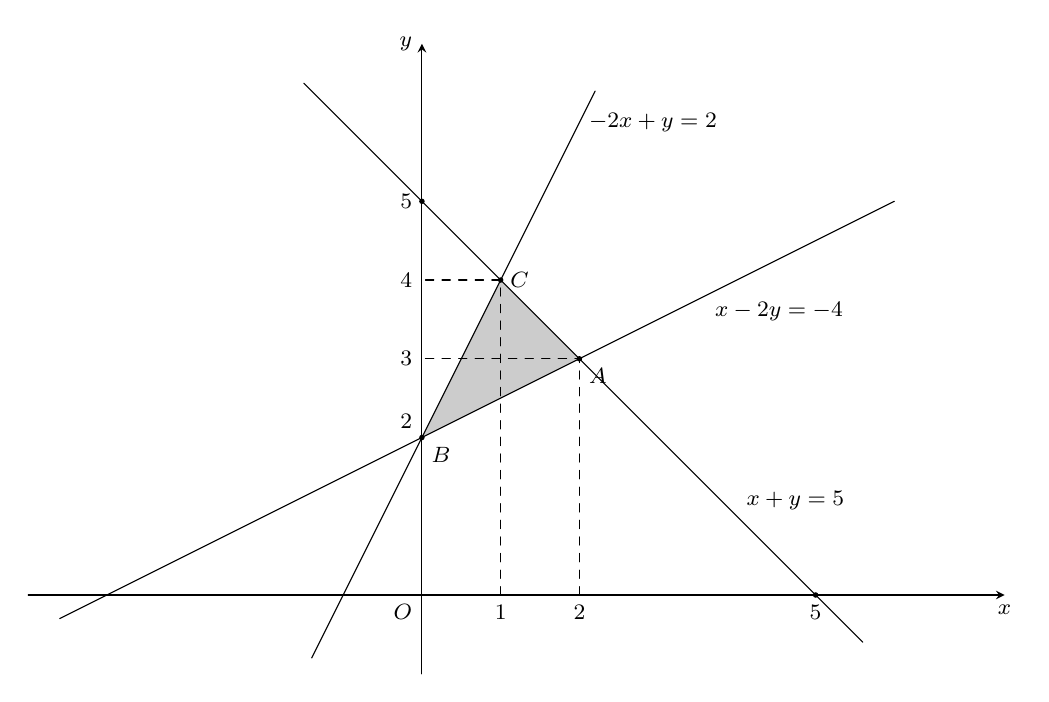
\begin{tikzpicture}[scale=1, font=\footnotesize, line join=round, line cap=round, >=stealth]
\draw plot[domain=-1.4:2.2] (\x,{2+2*\x});
\draw plot[domain=-1.5:5.6] (\x,{5-\x});
\draw plot[domain=-4.6:6] (\x,{(1/2)*(\x+4)});
\draw[->] (-5,0) -- (7.4,0) node[below] {$x$};
\draw[->] (0,-1) -- (0,7) node[left] {$y$};
\draw[dashed] (2,0)--(2,3)--(0,3);
\draw[dashed] (1,0)--(1,4)--(0,4);
\fill[opacity=0.2] (2,3) -- (0,2) -- (1,4) -- (2,3);
\fill (0,2) circle (1pt) node[below right] {$B$};
\fill (1,4) circle (1pt) node[right] {$C$};
\fill (2,3) circle (1pt) node[below right] {$A$};
\fill (5,0) circle (1pt) (0,5) circle (1pt);
\node[right] at (2,6) {$-2x+y=2$};
\node[right] at (3.6,3.6) {$x-2y=-4$};
\node[right] at (4,1.2) {$x+y=5$};
\node[below left] at (0,0) {$O$};
\node[below] at (1,0) {$1$};
\node[below] at (2,0) {$2$};
\node[below] at (5,0) {$5$};
\node[left] at (0,2.2) {$2$};
\node[left] at (0,3) {$3$};
\node[left] at (0,4) {$4$};
\node[left] at (0,5) {$5$};
\end{tikzpicture}
\end{center}
Suy ra, miền nghiệm của hệ bất phương trình $(1)$ là miền tam giác $ABC$ chứa $4$ điểm có tọa độ nguyên.
\itemch {\bf Đúng}.\\
Xét điểm $A(2;3)$, $F(2;3)=3-2=1$.\\
Xét điểm $B(0;2)$, $F(0;2)=2-0=2$.\\
Xét điểm $C(1;4)$, $F(1;4)=4-1=3$.\\
Vậy giá trị nhỏ nhất của $F(x;y)=y-x$ trên miền tam giác $ABC$ bằng $1$ (khi $x=2$, $y=3$).
\end{itemchoice}}
\end{ex}

% Phần II.Câu 2
\begin{ex}%[0-HK1-CD-6-NgocTao-HaNoi-2324]%[VN-MT-6, Bùi Lương Phúc]%[0H5H3-5]
Cho tam giác $MNP$, trên cạnh $NP$ lấy điểm $I$ sao cho $NI=3IP$. Qua $I$, kẻ đường thẳng $d_1$ song song với $MN$ cắt $MP$ tại $E$, kẻ đường thẳng $d_2$ song song với $MP$ cắt $MN$ tại $F$.
\choiceTF
{\True $\overrightarrow{MN}-\overrightarrow{MP}=\overrightarrow{PN}$}
{$\overrightarrow{MI}=\overrightarrow{ME}+\overrightarrow{MF}$}
{Nếu $\overrightarrow{IN}=k\overrightarrow{IP}$ thì $k=3$}
{\True Nếu $\overrightarrow{MI}=x\overrightarrow{MN}+y\overrightarrow{MP}$ thì $5x+y=2$}
\loigiai{
\begin{center}
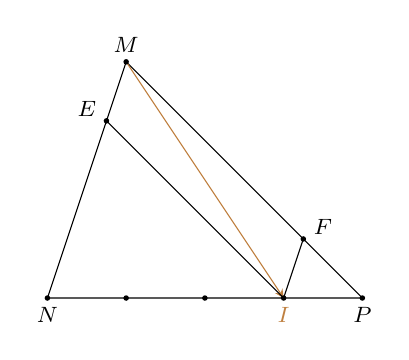
\begin{tikzpicture}[scale=1, font=\footnotesize, line join=round, line cap=round, >=stealth]
\coordinate (N) at (0,0);
\coordinate (P) at (4,0);
\coordinate (M) at (1,3);
\coordinate (I) at (3,0);
\coordinate (A) at (1,0);
\coordinate (B) at (2,0);
\coordinate (E) at (0.75,2.25);
\coordinate (F) at (3.25,0.75);
\draw (M) -- (N) -- (P) -- cycle;
\draw[brown,->] (M) -- (I) node[below] {$I$};
\draw (E) -- (I) -- (F);
\node at (0.5,2.4) {$E$};
\node at (3.5,0.9) {$F$};
\fill (N) circle (1pt) node[below] {$N$};
\fill (P) circle (1pt) node[below] {$P$};
\fill (M) circle (1pt) node[above] {$M$};
\fill (I) circle (1pt) (A) circle (1pt) (B) circle (1pt) (E) circle (1pt) (F) circle (1pt);
\end{tikzpicture}
\end{center}.
\begin{itemchoice}
\itemch {\bf Đúng}.\\
Theo công thức tính vectơ hiệu, ta có $\overrightarrow{MN}-\overrightarrow{MP}=\overrightarrow{PN}$.
\itemch {\bf Sai}.\\
Dễ thấy $MEIF$ là hình bình hành nên ta có $\overrightarrow{MI}=\overrightarrow{ME}+\overrightarrow{MF}$.
\itemch {\bf Sai}.\\
Ta có $\overrightarrow{IN}$ và $\overrightarrow{IP}$ ngược hướng và 	$\left|\overrightarrow{IN}\right|=3\left|\overrightarrow{IP}\right|$.\\
Vậy $\overrightarrow{IN}=-3\overrightarrow{IP}$ nên $k=-3$
\itemch {\bf Đúng}.\\
Theo định lý Thales, ta có \\
$ME=\dfrac{1}{4}MN$ nên $\overrightarrow{ME}=\dfrac{1}{4} \overrightarrow{MN}$.\\
$MF=\dfrac{3}{4}MP$ nên $\overrightarrow{MF}=\dfrac{3}{4} \overrightarrow{MP}$.\\
Vậy $\overrightarrow{MI}=\overrightarrow{ME}+\overrightarrow{MF}=\dfrac{1}{4} \overrightarrow{MN}+ \dfrac{3}{4} \overrightarrow{MP}$.\\
Suy ra $x=\dfrac{1}{4}$, $y=\dfrac{3}{4}$ nên $5x+y=2$.
\end{itemchoice}}
\end{ex}

% Phần II. Câu 3
\begin{ex}%[0-HK1-CD-6-NgocTao-HaNoi-2324]%[VN-MT-6, Bùi Lương Phúc]%[0D3H2-3]
Cho hàm số bậc hai $y=f(x)=ax^2+bx+c$ có đồ thị như hình vẽ bên.
\begin{center}
\begin{tikzpicture}[scale=1, font=\footnotesize, line join=round, line cap=round, >=stealth]
\draw[->] (-1,0) -- (7.3, 0) node[below] {$x$};
\draw[->] (0,-1) -- (0,2.5) node[left] {$y$};
\draw plot[domain=-0.3:4.3] (\x, {0.5*(\x-1)*(\x-3)});
\fill (0,0) circle (1pt) (1,0) circle (1pt) (3,0) circle (1pt);
\node[right] at (4.2,1.8) {$y=ax^2+bx+c$};
\node[below] at (1,0) {$1$};
\node[below] at (3,0) {$3$};
\node[below left] at (0,0) {$O$};
\end{tikzpicture}.\\
\end{center}
\choiceTF
{\True $f(x)=0\Leftrightarrow \hoac{&x=1 \\&x=3}$}
{Tập hợp các giá trị của $x$ để $f(x)$>0 là $(1;3)$}
{\True Trục đối xứng của đồ thị hàm số là đường thẳng $x=2$}
{$a>0$, $b>0$, $c>0$}
\loigiai
{\begin{itemchoice}
\itemch {\bf Đúng}.\\
Các hoành độ giao điểm của đồ thị với trục hoành là $x=1$ và $x=3$ cũng là nghiệm của phương trình $f(x)=0$.
\itemch {\bf Sai}.\\
Các giá trị của $x$ làm cho $f(x)>0$ ứng với phần trên trục hoành là $(-\infty;1)\cup (3;+\infty)$.
\itemch {\bf Đúng}.\\
Ta có $\dfrac{-b}{2a}=\dfrac{x_1 + x_2}{2}=\dfrac{1+3}{2}=2$.\\
Trục đối xứng của đồ thị hàm số là đường thẳng $x=\dfrac{-b}{2a}$ hay $x=2$.
\itemch {\bf Sai}.\\
Từ hình vẽ ta có $a>0$, $c>0$.\\
Ngoài ra, $\dfrac{-b}{2a}=2$ nên $b<0$.
\end{itemchoice}}
\end{ex}

% Phần II. Câu 4
\begin{ex}%[0-HK1-CD-6-NgocTao-HaNoi-2324]%[VN-MT-6, Bùi Lương Phúc]%[0D7H3-1]
Cho hai hàm số $f(x)=\sqrt{{{x}^{2}}+3x-2}$ và $g(x)=\sqrt{x+1}$. Gọi $A$ và $B$ lần lượt là tập xác định của các hàm số $f(x)$ và $g(x)$.
\choiceTF
{\True $f(2)=2\sqrt{2}$}
{$B=(-1;+\infty)$}
{\True $A\cap B=\left [\dfrac{-3+\sqrt{17}}{2};+\infty\right)$}
{Phương trình $f(x)=g(x)$ có hai nghiệm phân biệt}
\loigiai
{\begin{itemchoice}
\itemch {\bf Đúng}.\\
Thay $x=2$ vào biểu thức $f(x)$ ta được $f(2)=\sqrt{4+6-2}=2\sqrt{2}$.
\itemch {\bf Sai}.\\
Điều kiện xác định của $g(x)$ là $x+1\ge 0$ hay $x\ge -1$.\\
Vậy $B=[-1;+\infty)$.
\itemch {\bf Đúng}.\\
$A=\left(-\infty;\dfrac {-3-\sqrt{17}}{2}\right]\cup \left[\dfrac {-3+\sqrt{17}}{2};+\infty\right)$ nên $A\cap B=\left[\dfrac {-3+\sqrt{17}}{2};+\infty\right)$.
\itemch {\bf Sai}.\\
Phương trình $f(x)=g(x)\Rightarrow x^2+3x-2=x+1\Rightarrow x^2+2x-3=0\Rightarrow \hoac{&x=1 \\&x=-3.}$\\
Giá trị $x=-3$ không thỏa mãn phương trình.\\
Vậy phương trình đã cho có đúng một nghiệm là $x=1$.
\end{itemchoice}}
\end{ex}
\Closesolutionfile{ans}

%================================PHẦN III
\caukq
\Opensolutionfile{ans}[ans/0-HK1-CD-6-NgocTao-HaNoi-Phan-III]
\setcounter{ex}{0}
% Phần III. Câu 1
\begin{ex}%[0-HK1-CD-6-NgocTao-HaNoi-2324]%[VN-MT-6, Bùi Lương Phúc]%[0D7V2-3]
Bất phương trình $\left(5x-x^2\right)\sqrt{x^2-5x+6}>0$ có bao nhiêu nghiệm nguyên?
\shortans[]{$2$}
\loigiai
{Điều kiện xác định $x^2-5x+6\ge 0$ hay $\hoac{&x\ge 3 \\&x\le 2.}$\\
Từ điều kiện xác định và chiều của bất phương trình đã cho, ta phải có
$x^2-5x+6>0$ (1) và $5x-x^2>0$ (2).\\
Giải (1) ta được $\hoac{&x>3 \\&x<2.}$\\
Giải (2) ta được $0<x<5$.\\
Kết hợp lại ta được nghiệm của bất phương trình đã cho là $\hoac{&0<x<2 \\&3<x<5.}$\\
Vậy có hai giá trị nguyên của bất phương trình đó là $1$ và $4$.}
\end{ex}

% Phần III.Câu 2
\begin{ex}%[0-HK1-CD-6-NgocTao-HaNoi-2324]%[VN-MT-6, Bùi Lương Phúc]%[0H4H3-2]
\immini[thm]{Bạn Minh muốn đo khoảng cách từ vị trí $A$ bên bờ sông đến một vị trí $C$ ở bãi đất giữa sông. Minh bèn chọn một vị trí $B$ thích hợp bên bờ sông và thực hiện các phép đo đạc được kết quả như sau: $AB=100$\,m, $\widehat{A}=45^\circ$ và $\widehat{B}=70^\circ$ (tham khảo hình bên). Tính khoảng cách $AC$ (làm tròn kết quả đến hàng đơn vị).
}
%{
%%\begin{tikzpicture}[scale=1, font=\footnotesize, line join=round, line cap=round, >=stealth]
%%\draw (0,0) node[left] {$B$} -- (6,0) node[right] {$A$} --
%%(2,4) node[above] {$C$} -- cycle;
%%\draw (2,4) -- (0,0);
%%\draw (2,4) -- (6,0);
%%\draw (0.5,0) arc[start angle=0,end angle=65,radius=0.5] node[midway,right] {70$^\circ$};
%%\draw (5.5,0) arc[start angle=180,end angle=160,radius=1.2]
%%node[midway,left] {45$^\circ$};
%%\draw (5.6,0) arc[start angle=180,end angle=160,radius=1];
%%\node at (3,-0.3) {100 m};
%%\fill[gray!30] (2.5,3.5) ellipse (1.3cm and 0.7cm);
%%\fill[red] (2,4) circle (1pt);
%%\end{tikzpicture}
%}
{	\definecolor{lightcornflowerblue}{rgb}{0.05, 1, 1}
	\definecolor{cadmiumgreen}{rgb}{0.0, 0.6, 0.3}
	\definecolor{trueblue}{rgb}{0.0, 0.6, 0.9}
	\definecolor{tumbleweed}{rgb}{0.87, 0.7, 0.6}%màu cát
	\begin{tikzpicture}[line join=round, line cap=round,scale=1,transform shape]
		
		%Vẽ đảo
		\tikzset{dao/.pic={
				\def\H{ 
					(-0.3,1.3)
					..controls +(60:0) and +(90:0.1) .. (0,1.3)
					..controls +(60:.1) and +(140:0) .. (0,1.3)
					..controls +(10:.6) and +(120:0.2) .. (1,1.1)
					..controls +(-50:.2) and +(0.1:0.4) .. (.1,1)
					..controls +(-140:.3) and +(-10:0.2) .. (-0.4,1.2)
					..controls +(70:.2) and +(-20:0.3) .. cycle
					;}
				\draw \H;
				\fill[tumbleweed] \H;
		}}
		
		%Vẽ núi
		\tikzset{nui/.pic={
				\def\T{ %Trời
					(-3.65,1.75)
					..controls +(60:.05) and +(-160:0) .. (-3.4,1.8)
					..controls +(45:.1) and +(-150:0) .. (-3.1,1.78)
					..controls +(45:.1) and +(-150:0) .. (-2.7,1.75)
					..controls +(60:.1) and +(-160:0) .. (-2.4,1.8)
					..controls +(60:.1) and +(-160:0) .. (-1.45,1.74)
					..controls +(60:.1) and +(-160:0) .. (-.4,1.64)
					..controls +(30:.1) and +(160:0.1) .. (.98,1.74)
					..controls +(40:.1) and +(130:0.1) .. (2.2,1.76)
					..controls +(30:.1) and +(150:0.1) .. (3,1.8)
					..controls +(10:.1) and +(170:0.1) .. (3.66,1.78)--(3.66,1.95)--(-3.65,1.95)--cycle
					;}
				\draw \T;
				\fill[lightcornflowerblue] \T;
				\def\N{ 
					(-3.65,1.75)
					..controls +(60:.05) and +(-160:0) .. (-3.4,1.8)
					..controls +(45:.1) and +(-150:0) .. (-3.1,1.78)
					..controls +(45:.1) and +(-150:0) .. (-2.7,1.75)
					..controls +(60:.1) and +(-160:0) .. (-2.4,1.8)
					..controls +(60:.1) and +(-160:0) .. (-1.45,1.74)
					..controls +(60:.1) and +(-160:0) .. (-.4,1.64)
					..controls +(30:.1) and +(160:0.1) .. (.98,1.74)
					..controls +(40:.1) and +(130:0.1) .. (2.2,1.76)
					..controls +(30:.1) and +(150:0.1) .. (3,1.8)
					..controls +(10:.1) and +(170:0.1) .. (3.66,1.78)--(3.66,1.16)
					..controls +(175:.2) and +(20:0) .. (0,1.5)
					..controls +(20:0) and +(20:.7) .. (-3.65,1.28)--cycle
					;}
				\draw \N;
				\fill[cadmiumgreen] \N;
		}}
		
		%Vẽ biển
		\tikzset{bien/.pic={
				\def\B{ 
					(3.66,1.16)
					..controls +(175:.2) and +(20:0) .. (0,1.5)
					..controls +(20:0) and +(20:.7) .. (-3.65,1.28)--(-3.65,-.65)
					..controls +(15:.2) and +(120:0) .. (0,-.62)
					..controls +(-60:0) and +(-160:0.1) .. (3.66,-.65)--(3.66,1.16)
					;}
				\draw \B;
				\fill[trueblue!70!] \B;
				\def\C{ %Cát
					(-3.65,-.65)
					..controls +(15:.2) and +(120:0) .. (0,-.62)
					..controls +(-60:0) and +(-160:0.1) .. (3.66,-.65)--(3.66,-1.9)--(-3.65,-1.9)--cycle
					;}
				\draw \C;
				\fill[tumbleweed] \C;
		}}
		%Vẽ người
		\tikzset{nguoi/.pic={
				\def\N{ 
					(-3.04,-.64)--(-3.025,-.6)
					..controls +(90:.1) and +(85:0.06) .. (-3.122,-.59)--(-3.11,-.63)
					..controls +(-160:.07) and +(110:0.05) .. (-3.14,-.81)
					..controls +(-40:.01) and +(60:0) .. (-3.14,-.85)
					..controls +(-120:.07) and +(80:0.05) .. (-3.16,-1.1)
					..controls +(-120:.09) and +(80:0.05) .. (-3.18,-1.28)
					..controls +(-120:.02) and +(170:0.01) .. (-3.165,-1.318)--(-3.1,-1.31)--(-3.1,-1.29)
					..controls +(120:.01) and +(-30:0) .. (-3.135,-1.278)
					..controls +(120:.02) and +(-120:0.04) .. (-3.1,-1.1)
					..controls +(-70:.04) and +(120:0.01) ..(-3.096,-1.14)
					..controls +(-120:.04) and +(120:0.01) ..(-3.09,-1.3)
					..controls +(-120:.02) and +(170:0.02) .. (-3.08,-1.34)--(-2.98,-1.34)
					..controls +(70:.03) and +(-70:0.01) .. (-3.045,-1.296)
					..controls +(110:.04) and +(-70:0.01) .. (-3.03,-1.1)
					..controls +(70:.03) and +(-100:0.01) .. (-3.014,-1.04)--(-3,-1.02)
					..controls +(70:.03) and +(-100:0.01) .. (-3.014,-.85)--(-2.97,-.84)
					..controls +(40:.04) and +(-10:0) .. (-2.98,-.7)
					..controls +(110:.04) and +(-20:0.02) .. (-3.043,-.66)--cycle
					;}
				\draw \N;
				\fill[black!70!] \N;
				\def\Q{ %quần
					(-3.045,-.9)
					..controls +(120:.01) and +(-30:0) .. (-3.04,-1.04)
					-- (-3.1,-1.038)
					..controls +(80:.07) and +(-10:0.01) .. (-3.13,-.94)--(-3.124,-.9)--cycle
					(-3.14,-1.04)--(-3.12,-1.04)
					..controls +(80:.07) and +(-10:0.01) .. (-3.134,-.96)--cycle
					;}
				%\draw \Q;
				\fill[green] \Q;
				
		}}
		
		
		\path
		(0,0)pic[scale=1]{bien} (0,0)pic[scale=1]{dao}
		(0,0)pic[scale=1]{nui}
		(0,0)pic[scale=1]{nguoi} (-1.1,0)pic[scale=1,rotate=180,yscale=-1]{nguoi}
		;
		
		\draw[dashed] (1.9,-.6) node[above] {\tiny $B$}--(-.1,1.1)node[right] {\tiny $C$}--(-3,-.54)node[above] {\tiny $A$};
		\draw (-2.6,-.46)--(-2.45,-.4);%gạch góc
		\draw[<->,red,line width=1] (-3,-.6)--(1.9,-.6);
		\node at (-.5,-.7) [below]{\tiny $500$ m};
		\node at (1,0.2) [above]{\tiny $?$};
		\node at (-2.2,-.6) [above]{\tiny $60^\circ$};
		\node at (1.3,-.6) [above]{\tiny $70^\circ$};
		%góc
		\draw (-2.6,-.3)
		..controls +(-50:.09) and +(60:0.01) .. (-2.5,-.6);
		\draw[scale=1,rotate=180,xscale=.6,yscale=-1] (-2.6,-.3)
		..controls +(-50:.09) and +(70:.2) .. (-2.5,-.6);
\end{tikzpicture}}
\shortans[]{$104$}
\loigiai{
Trong tam giác $ABC$ ta có $\widehat{C}=180^\circ-\widehat{A}-\widehat{B}=65^\circ$.\\
Theo định lý sin, ta có 
\[\dfrac{AB}{\sin C}=\dfrac{AC}{\sin B}
\Rightarrow AC=\dfrac{AB\cdot\sin B}{\sin C}
=\dfrac{100\cdot\sin 70^\circ}{\sin 65^\circ}\approx 104.\]
Vậy $AC=104$ m.
}
\end{ex}

% Phần III. Câu 3
\begin{ex}%[0-HK1-CD-6-NgocTao-HaNoi-2324]%[VN-MT-6, Bùi Lương Phúc]%[0H5V2-6]
Một máy bay đang bay từ hướng Đông sang hướng Tây với tốc độ $650$ km/h thì gặp luồng gió thổi từ hướng Đông Bắc sang hướng Tây Nam với vận tốc $35$ km/h. Máy bay bị thay đổi vận tốc sau khi gặp gió thổi.
\begin{center}
\begin{tikzpicture}[scale=1, font=\footnotesize, line join=round, line cap=round, >=stealth]
\foreach \a/\text in {0/Đông, 45/Đông Bắc, 90/Bắc, 135/Tây Bắc, 180/Tây, 225/Tây Nam, 270/Nam, 315/Đông Nam} {
\draw[->] (0,0) -- (\a:1.8);
\node at (\a:2.4) {\text};}
\end{tikzpicture}
\\
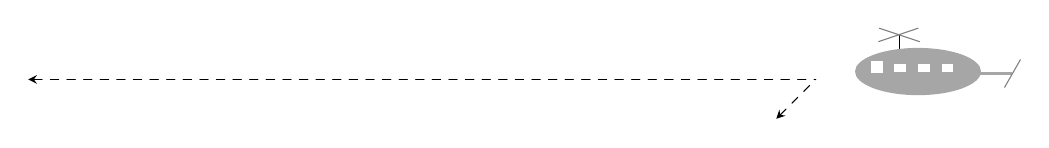
\begin{tikzpicture}[scale=1, font=\footnotesize, line join=round, line cap=round, >=stealth]
\draw[dashed, <-] (3,0) -- (13,0);
\draw[dashed, <-] (12.5,-0.5) -- (13,0);
\draw (14.06,0.36) -- (14.06,0.56);
\draw[gray] (13.8,0.48) -- (14.3,0.65);
\draw[gray] (13.81,0.65) -- (14.32,0.48);
\fill[gray!70] (15.05,0.05) rectangle (15.5,0.1);
\draw[gray] (15.4,-0.1) -- (15.6,0.25);
\fill[gray!70] (14.3,0.1) ellipse (0.8cm and 0.3cm);
\fill[white] (13.7,0.08) rectangle (13.85,0.23);
\fill[white] (14,0.1) rectangle (14.15,0.2);
\fill[white] (14.3,0.1) rectangle (14.45,0.2);
\fill[white] (14.6,0.1) rectangle (14.75,0.2);
\end{tikzpicture}
\end{center}
Tìm tốc độ mới của máy bay (kết quả làm tròn đến hàng đơn vị, đơn vị: km/h)?
\shortans[]{$675$}
\loigiai
{Dựng hình bình hành $MNPQ$ thỏa mãn $\left|\overrightarrow{MN}\right|=650, \left|\overrightarrow{MQ}\right|=35$.\\
\begin{center}
\begin{tikzpicture}[scale=1, font=\footnotesize, line join=round, line cap=round, >=stealth]
\coordinate (M) at (13.3,0);
\coordinate (N) at (6.8,0);
\coordinate (Q) at (11.8,-1.5);
%\coordinate (N1) at (0.3,0);
%\coordinate (Q1) at (12.8,-0.5);
%\coordinate (N) at ($(M)!1/2!(N1)$);
%\coordinate (Q) at ($(M)!3!(Q1)$);
\coordinate (P) at (5.3,-1.5);
\draw[dashed, ->] (M) -- (N) (M)--(Q);
\draw[dashed] (N)--(P)--(Q);
\draw[->, blue] (M)--(P);
\foreach \x/\y in {M/90,N/90,P/-90,Q/-90} \fill[black](\x) circle (1pt) ($(\x)+(\y:3mm)$) node{$\x$};
\end{tikzpicture}
\end{center}

Khi đó hướng bay và vận tốc mới của máy bay chính là vectơ $\overrightarrow{MP}$.\\
Theo định lý cosin trong tam giác $MNP$, ta có
\[MP=\sqrt{MN^2+MQ^2-2\cdot MN\cdot MQ\cdot \cos 135^\circ}=\sqrt{423725+22750\sqrt{2}}\approx 675.\]
Tốc độ mới của máy bay là $675$ km/h.
}
\end{ex}

% Phần III. Câu 4
\begin{ex}%[0-HK1-CD-6-NgocTao-HaNoi-2324]%[VN-MT-6, Bùi Lương Phúc]%[0D3V2-2]
Có bao nhiêu giá trị nguyên dương của tham số $m$ để hàm số $y=-x^2+2(3m-6)x+3-5m$ nghịch biến trên khoảng $(6;2\,023)$?
\shortans[]{$4$}
\loigiai
{Hàm số đã cho là hàm số bậc hai có hệ số $a<0$ nên nó nghịch biến trên khoảng $(3m-6;+\infty)$.\\
Để thỏa mãn yêu cầu bài toán thì phải có $3m-6\le 6$ hay $m\le 4$.\\
Vậy có bốn giá trị nguyên dương của $m$ thỏa mãn, đó là $1$, $2$, $3$, $4$.}
\end{ex}

% Phần III. Câu 5
\begin{ex}%[0-HK1-CD-6-NgocTao-HaNoi-2324]%[VN-MT-6, Bùi Lương Phúc]%[0D3V1-3]
Bảng niêm yết giá cước của một hãng taxi như sau:
\begin{center}
\begin{tabular}{|c|c|c|}
\hline
Giá mở cửa	&Giá km tiếp theo &Từ km thứ $26$\\
\hline
$14\,000$ đ/$0{,}8$km	&$16\,300$ đ/km &$13\,300$ đ/km \\
\hline
\end{tabular}
\end{center}
Bác An đi taxi và cần di chuyển quãng đường $20$ km. Hỏi bác An phải trả bao nhiêu tiền?
(kết quả làm tròn tới hàng nghìn, đơn vị: nghìn đồng)
\shortans[]{$327$}
\loigiai
{Cần chi $14\,000$ đồng cho $0{,}8$ km đầu tiên;\\
$16\,300\cdot (205-0,8)=312\,960$ đồng cho những km tiếp theo của quãng đường $20$ km.\\
Tổng số tiền bác An phải trả là $14\,000 + 312\,960 = 326\,960$ đồng.}
\end{ex}

% Phần III.Câu 6
\begin{ex}%[0-HK1-CD-6-NgocTao-HaNoi-2324]%[VN-MT-6, Bùi Lương Phúc]%[0D3V2-6]
Bộ phận nghiên cứu thị trường của một xí nghiệp xác định tổng chi phí để sản xuất $x$ sản phẩm là $f(x)=\dfrac {x^2}{1\,000} + \dfrac{x}{5} + 190$ (triệu đồng). Giả sử giá mỗi sản phẩm bán ra thị trường là $2$ triệu đồng. Xác định lợi nhuận xí nghiệp thu được sau khi bán hết $500$ sản phẩm. (Lợi nhuận là hiệu của doanh thu trừ đi tổng chi phí để sản xuất, đơn vị: triệu đồng).
\shortans[]{$460$}
\loigiai
{Doanh thu $2\cdot 500=1\,000$.\\
Tổng chi phí $f(500)=\dfrac{500^2}{1\,000}+\dfrac {500}{5} +190=540$.\\
Lợi nhuận $1\,000-540=460$ triệu đồng.
}
\end{ex}
\Closesolutionfile{ans}
% \begin{indapan}
% 	{ans/0-HK1-CD-6-NgocTao-HaNoi}
% \end{indapan}



